\lez{16}{25-03-2020}{}
\subsection{Introduzione ai solidi.}
\label{subsec:Solidi}
\subsubsection{Hamiltoniana di un solido.}%
\label{subsub:Hamiltoniana di un solido.}

I solidi sono in genere sistemi molto complicati: nuclei, elettroni interagiscono tra di loro. In linea di principio possiamo scrivere una Hamiltoniana e trovare le sue Autofunzioni.
\[
	H \psi = E \psi
.\] 
Tale Hamiltoniana ha tantissimi contributi:
\[
	H = T_e + T_N + V_{N-N} + V_{N-e} + V_{e-e} + C_e^{\text{rel}}
.\] 
Nella quale:
\begin{description}
	\item[Termine cinetico per gli elettroni] 
		 \[
			T_e = \sum_{e}^{} \frac{p_e^2}{2m} 
			= -\sum_{e}^{} \frac{\hbar ^2 \nabla_i^2}{2m}
		.\] 

	\item[Termine cinetico per i nuclei] 
		\[
			T_N 
			=
			-\sum_{I}^{} \frac{\hbar ^2 \nabla_{R_I}^2}{2M}
		.\] 
	\item[Termine di interazione Nucleo-Nucleo]
		\[
			V_{N-N} = 
			\frac{1}{2}\sum_{i\neq j}^{} 
			\frac{Z_iZ_je^2}{\left| R_i - R_j \right| }
		.\]  
	\item[Termine di interazione elettrone-elettrone]
		\[
			V_{e-e} = 
			\frac{1}{2}\sum_{i\neq j}^{} 
			\frac{e^2}{\left| r_i - r_j \right| }
		.\]
	\item[Termine di interazione Nucleo-elettrone]
		\[
			V_{N-e} = 
			\frac{1}{2}\sum_{i,I}^{} 
			\frac{Z_ie^2}{\left| r_i - r_j \right| }
		.\]
	\item[Correzioni relativistiche per gli elettroni]
		\[
			C_e^{\text{rel}} 
			=
			\sum_{e}^{} \left[ \underbrace{-\frac{p_e^4}{2m^3c^2}}_
			{\substack{\text{Correzione al}\\ 
			\text{primo ordine}\\ 
			\text{su $T_e$}}}
			+ 
			\underbrace{\frac{\hbar ^2 \nabla_e^2 V_e}{8m^2c^2}}_
			{\substack{\text{L'elettrone vede}\\
			\text{un potenziale}\\
			\text{medio esteso su}\\
			\text{una certa dim.}}}
			+
			\underbrace{\frac{\hbar }{4m^2c^2}
			\left( \nabla \bs{v}_e \wedge\bs{p}_e\right) 
			\bs{\sigma}_e}_
			{\substack{\text{Termine}\\
			\text{Spin-Orbita}}}
			\right] 
		.\] 
		Il termine spin orbita deriva dal fatto che un elettrone che si muove
		all'interno di un campo elettrico vede nel suo sistema di riferimento
		un campo magnetico:
		\[
			\bs{B} = -\frac{\bs{v}\wedge \bs{E}}{c}
		.\] 
		l'elettrone ha un momento magnetico:
		\[
			\bs{\mu} = - \frac{e\hbar }{2mc} \bs{\sigma}_e
		.\] 
		Dove il termine $\v{\sigma}_e$ è proporzionale allo spin. In conclusione otteniamo:
		\[
			-\bs{B}\bs{\mu} 
			=
			\frac{\hbar ^2}{2m^2c^2}\left( \nabla v_e \wedge \bs{p}_e \right)
			\bs{\sigma}_e
		.\] 
\end{description}
\subsubsection{Approssimazione di Born-Oppenheimer.}%
\label{subsub:Approssimazione di Born-Oppenheimer.}
Risolvere una Hamiltoniana del genere in modo esplicito è un grosso casino viste le dipendenze di ognuno dei termini precedenti:
\[
    H(\left\{ \bs{r} \right\}, \left\{ \bs{R} \right\}) \psi (\left\{\v{r}\right\}, \left[\v{R}\right]) 
	=
	E \psi(\left\{ \bs{r} \right\} , \left\{ \bs{R} \right\} )
.\] 
Per risolvere questo problema facciamo la seguente approssimazione:
\begin{fact}[Approssimazione adiabatica o di Born-Oppenheimer]{fact:Approssimazione adiabatica o di Born-Oppenheimer}
L'approssimazione adiabatica o di Born-Oppenheimer consiste nel supporre il moto dei nuclei molto più lento di quello degli elettroni.
\end{fact}
L'obbiettivo è risolvere il moto degli elettroni avendo assunto i nuclei atomici statici nelle loro posizioni reticolari.
A tale scopo si scrive la funzione d'onda nel seguente modo:
\[
	\psi(\left\{ \bs{r} \right\}, \left\{ \bs{R} \right\} )
	=
	\underbrace{F(\left\{ \bs{R} \right\})}_
	{\substack{\text{Moto nuclei}}}
	\underbrace{\varphi(\left\{\bs{r}\right\},\left\{\bs{R}\right\} )}_
	{\substack{\text{Moto elettroni}}}
.\] 
Sostituendo questa nella Hamiltoniana i termini riguardanti gli elettroni restano invariati, il termine cinetico nucleare invece cambia nel Laplaciano:
\[\begin{aligned}
& 			&		&\varphi(\left\{ \bs{r} \right\}, \left\{ \bs{R} \right\}) \ \nabla^2_R F(\left\{ R \right\} ) +\\
\nabla^2_R \psi&\to 	& 		&\cancel{2\nabla_RF(\left\{\bs{R}\right\}) \ \nabla_R\varphi(\left\{ \bs{r} \right\},\left\{ \bs{R} \right\} )}+\\
&			&		&\cancel{F(\left\{ \bs{R} \right\} ) \ \nabla_R^2\varphi(\left\{ \bs{r} \right\},\left\{ \bs{R} \right\} )}
.\end{aligned}\]
L'approssimazione consiste nel trascurare i termini in cui vi è la derivata rispetto a $\bs{R}$ di $\varphi$. Questo significa considerare nella $\varphi$ le coordinate dei nuclei fissati.\\
L'equazione di Schrodinger diventa:
\[\begin{aligned}
	&-\frac{\hbar ^2}{2m}F(\bs{R})\nabla _r^2\varphi(\bs{R},\bs{r}) +\\
	&+\left( V_{ee} + V_{eN} + C_e^{\text{rel}} \right)
	F(\bs{R})\varphi(\bs{R},\bs{r})+\\
	&- \frac{\hbar ^2}{2M}\varphi(\bs{r},\bs{R})\nabla_R^2F(\bs{R}) +\\
	&+V_{NN}F(\bs{R})\varphi(\bs{r},\bs{R}) =\\
	&=EF(\bs{R})\varphi(\bs{r},\bs{R})
.\end{aligned}\]
Cerchiamo di renderla separabile: dividiamo per la funzione d'onda stessa. Abbattendo ulteriormente la notazione possiamo scrivere:
\[
	-\frac{\hbar ^2}{2m}\frac{\nabla_r^2\varphi}{\varphi} +
	V_{ee} + V _{eN} + C_e^{\text{rel}} -
	\frac{\hbar ^2}{2M}\frac{\nabla_R^2F}{F} = E
.\] 
A questo punto l'ultimo termine prima dell'uguale è solo una costante per gli elettroni, non contribuirà alla distribuzione dei livelli energetici se non come un offset, quindi abbiamo che possiamo risolvere per le energie dei livelli elettronici $E_n(\bs{R})$ nel potenziale dei nuclei:
\[
	-\frac{\hbar ^2}{2m}
	\frac{\nabla_r^2 \varphi(\bs{r},\bs{R})}{\varphi(\bs{r},\bs{R})} +
	V_{eN} + V_{ee} + C_e^{\text{rel}} = E_n(\bs{R})
.\] 
Oppure possiamo riscriverla meglio come:
\[
	-\frac{\hbar ^2}{2m}
	\nabla_r^2 \varphi(\bs{r},\bs{R}) +
	\left( V_{eN} + V_{ee} + C_e^{\text{rel}} \right)
	\varphi(\bs{r},\bs{R}) = E_n(\bs{R})\varphi(\bs{r}, \bs{R})
.\] 
Trovate le soluzioni per gli elettroni possiamo sostituire per la parte di equazione che risolveva i nuclei:
\[
	-\frac{\hbar ^2}{2M}\nabla_R^2F(\bs{R})+
	\left[ V_{NN}+E_n(\bs{R}) \right] F(\bs{R})=
	E F(\bs{R})
.\] 
Senza il funzionale $E_n$ il cristallo non starebbe insieme: tutti gli altri termini in equazione sono repulsivi.\\
Risolvere l'equazione per gli elettroni è molto complicato, dobbiamo semplificare ancora per ricavarne qualche informazione: scriviamo la funzione d'onda per gli N elettroni come un prodotto di funzioni d'onda a singolo elettrone. É necessario ricordare che gli elettroni sono fermioni quindi tale prodotto deve essere antisimmetrico:
\[
	\varphi(\bs{r},\bs{R}) =
	\frac{1}{\sqrt{n!}}
	\begin{vmatrix}
		\varphi_1(r_1) 	& \ldots 	& \varphi_1(r_n)\\
		\ldots		& \ldots	&\ldots	\\
		\varphi_n(r_1)	&\ldots		& \varphi_n(r_n)
	\end{vmatrix}
.\] 
Il determinante nella precedente equazione così definito descrive il prodotto antisimmetrico richiesto e si chiama determinante di Slater.
Sostituendo questa troveremo una Hamiltoniana a singola particella:
\[
	H_{F}(r_i)\varphi_i(r_i) = 
	E_i \varphi_i(r_i)
.\] 
Utilizzando l'approssimazione di Born-Oppenheimer ci siamo persi le interazioni tra gli elettroni ed i modi di vibrazione de cristallo, ovvero i fononi\footnote{Questa interazione la vedrà chi affrontera stato solido.}.\\
Abbiamo iniziato a cercare soluzioni indipendenti, quindi abbiamo spezzato la funzione d'onda dipendente dalle variabili degli $n$ elettroni nel prodotto di $n$ funzioni d'onda dipendenti ognuna dalle variabili del proprio elettrone. Per far questo abbiamo trovato la formula con il determinante di Slater.
Prendiamo il prodotto antisimmetrizzato così ottenuto e lo inseriremo nella Hamiltoniana, proiettiamo inoltre su una singola $\psi$: 
\[
	H_{HF}(\bs{r}_i)\psi_i(\bs{r}_i) 
	=
	E_i \psi_i(\bs{r}_i)
.\] 
Esplicitando l'Hamiltoniana si ha:
\[\begin{aligned}
	&-\frac{\hbar^2}{2m}\nabla^2\psi_i(\bs{r}) -
%
	\underbrace{-\sum_{I}^{} 
		\frac{Z_i e^2}{\left| \bs{r}-\bs{R} \right| }
		\psi_i (\bs{r})}_
		{\text{Interazione con nuclei}} +
%
	\underbrace{
		\left[ \sum_{j\neq i}^{} 
		e^2\int
		\frac{\psi_j^*(\bs{r}')\psi_j(\bs{r}')}{\left| \bs{r}-\bs{r}' \right| }
		d \bs{r}' \right] \psi_i(\bs{r})}_
		{\text{Repulsione Columbiana}}+\\
%
	&\underbrace{
		-\left[ \sum_{j}^{} e^2\left( \int \frac{\psi_j^*(\bs{r}')
		\psi_j(\bs{r}')}{\left| \bs{r}-\bs{r}'\right|}d\bs{r}'\right)
		\psi_j(\bs{r})\right]}_
		{\text{Termine di scambio}} =
	E_i \psi_i(\bs{r})
.\end{aligned}\]
Il termine di scambio viene fuori dall'aver antisimmetrizzato la funzione d'onda.\\
Vediamo adesso come trattare i vari termini della equazione. Per il termine Coulombiano è semplice, possiamo trattarlo come una densità di elettroni dicendo che:
\[
	\sum_{i=1}^{n} \left| \psi_i(\bs{r}) \right| ^2=n(\bs{r})
.\] 
In questo modo il contributo alla Hamiltoniana diventa:
\[
	\int\frac{e^2n(\bs{r})}{\left| \bs{r}-\bs{r}' \right| }d \bs{r}
.\] 
tuttavia non conosciamo la densità degli elettroni in generale, una buona approssimazione consiste nel partire dalla somma delle densità degli elettroni prendendo come funzioni d'onda gli orbitali atomici. In questo modo troveremo un potenziale $U(\bs{r})$ da inserire nella Hamiltoniana. \\
Per trattare il termine di scambio solitamente si utilizza un metodo detto Local Density: prendere la media sulle funzioni d'onda di $U(\bs{r})$ e per calcolarlo utilizzare come funzioni d'onda quelle gli elettroni liberi (onde piane).\\
Senza trattare questo metodo diciamo soltanto che alla fine del procedimento si arriva ad un problema Hamiltoniano di singola particella:
\[
	H = -\frac{\hbar ^2}{2m}\nabla^2 + U_c(\bs{r})
.\] 
Dove $U_c(\bs{r})$ è un potenziale che viene fuori dai vari termini introdotti sopra.\\
La soluzione che si ottiene con questo metodo è una soluzione ad elettroni indipendenti: ci sarà comunque un termine di interazione elettrone-elettrone ma non saremo in grado di trovare le correlazioni tra gli elettroni.

\subsection{Reticoli nei solidi}
\label{subsec:Reticoli nei solidi}
Supponiamo che gli ioni del solido siano disposti in modo ordinato come celle che si ripetono nello spazio, in questo modo possiamo considerare $U_c(\bs{r})$ periodico.\\
Visto che il cristallo ha una struttura di questo tipo possiamo descriverlo con un reticolo: un insieme di vettori $\bs{R}$ che definiscono nello spazio le posizioni di ciascuno ione. In 3 dimensioni possiamo scrivere un vettore di base del reticolo come:
\[
	\bs{R} = n_1 \bs{a}_1 + n_2 \bs{a}_2 + n_3 \bs{a}_3	
.\] 
Dove gli $n_i$ sono numeri interi mentre gli $\bs{a}_i$ sono detti vettori primari, questi ultimi ci identificano la cella unitaria del reticolo.
\begin{figure}[ht]
    \centering
    \incfig{esempio-di-reticolo}
    \caption{Esempio di reticolo}
    \label{fig:esempio-di-reticolo}
\end{figure}
La cella in Figura \ref{fig:esempio-di-reticolo} sottesa ai vettori primari è detta cella unitaria.
La scelta della cella unitaria per il reticolo è arbitraria, l'unico criterio da rispettare è che sia effettivamente la più piccola per preservare la periodicità. Infatti avremmo potuto tranquillamente prendere i vertici del reticolo coincidenti con gli atomi come in \ref{fig:reticolo-alternativo}.
\begin{figure}[ht]
    \centering
    \incfig{reticolo-alternativo}
    \caption{Reticolo alternativo}
    \label{fig:reticolo-alternativo}
\end{figure}
Un altro esempio potrebbe essere quello della grafite, questa ha una struttura esagonale, il più piccolo reticolo che si può fare per preservare la periodicità nel caso della grafite è composto da due atomi.
\begin{defn}[Reticolo di Bravais]{def:Reticolo}
	Insieme di vettori che descrivono la struttura periodica del cristallo.
\end{defn}
Per descrivere il cristallo possiamo introdurre un ulteriore reticolo: $\bs{K}$. Questo è l'insieme dei vettori che soddisfano
\[
	e^{i \bs{K}\cdot\bs{R}}=1 \label{eq:Bravet-rel}
.\] 
Anche questi vettori $\bs{K}$ formano un reticolo di Bravais, questo è detto \textit{Reticolo reciproco}:
\[
	 \bs{K}=m_1\bs{b}_1 + m_2\bs{b}_2 + m_3\bs{b}_3
.\] 
Soddisfare la relazione \ref{eq:Bravet-rel} implica che deve esser vera anche la seguente:
\[
	\bs{b}_i \cdot  \bs{a}_j=2\pi\delta_{ij}
.\] 
\subsubsection{Esempio: reticolo cubico}
\label{subsubsec:Esempio: reticolo cubico}
Nel caso di reticolo cubico abbiamo che la relazione sopra si scrive come:
\[\begin{aligned}
	&\bs{a}_1=a \hat{x}&&		&\bs{b}_1=\frac{2\pi}{a}\hat{x}\\
	&\bs{a}_2=a \hat{y}&&		&\bs{b}_2=\frac{2\pi}{a}\hat{y}\\
	&\bs{a}_3=a \hat{z}&&		&\bs{b}_3=\frac{2\pi}{a}\hat{z}
.\end{aligned}\]
Il reticolo reciproco è quindi anche esso cubico, non è scontato in generale che tale reticolo assuma la stessa forma del reticolo diretto.\\
In genere si usa una particolare cella chiamata Zona di Brilloiun.
\subsection{Prima zona di Brilloiun}
\label{subsec:Zona di Brilloiun}
Dato il reticolo reciproco prendiamo tutti i vettori $\bs{K}$ e se ne costruiscono le rette che bisecano tali vettori, l'area generata dalle bisecanti è la prima zona di Brilloiun. Vediamo che forma ha nel caso di un reticolo quadrato bidimensionale in Figura \ref{fig:zona-di-brilloiun-per-reticolo-quadrato-bidimensionale}
\begin{figure}[ht]
    \centering
    \incfig{zona-di-brilloiun-per-reticolo-quadrato-bidimensionale}
    \caption{\scriptsize Zona di Brilloiun per reticolo quadrato bidimensionale partendo
    dal reticolo diretto.}
    \label{fig:zona-di-brilloiun-per-reticolo-quadrato-bidimensionale}
\end{figure}
Questo metodo e la cella che ne deriva hanno un nome famoso: \textit{cella primitiva di Wiegner-Seitz}.
Quindi nel reticolo reciproco la cella di Wiegner-Seitz è detta anche prima zona di Brilloiun.\\
I vettori del reticolo reciproco assumono un ruolo molto importante nella descrizione degli stati elettronici, hanno inoltre una connessione diretta con gli esperimenti che possiamo fare per studiare la struttura del cristallo.

\subsection{Osservazione della struttura periodica del cristallo}
\label{subsec:Osservazione della struttura periodica del cristallo}
Per osservare la struttura periodica del materiale ad inizio secolo vennero fatti esperimenti con i raggi X, per schematizzare questi esperimenti di diffrazione prendiamo un solido avente un atomo per cella, la distanza tra gli atomi è $a$ come in Figura \ref{fig:esperimento-per-osservazione-struttura-cristallo}. Su questo reticolo mandiamo un'onda elettromagnetica che viene scatterata dal cristallo ineragendo con gli atomi.
\begin{figure}[ht]
    \centering
    \incfig{esperimento-per-l'ossevazione-della-struttura-periodica-dei-cristalli}
    \caption{Esperimento per l'ossevazione della struttura periodica dei cristalli}
    \label{fig:esperimento-per-osservazione-struttura-cristallo}
\end{figure}
Cerchiamo l'interferenza costruttiva della radiazione dopo il passaggio attraverso il cristallo. Dallo schema di Figura \ref{fig:esperimento-per-osservazione-struttura-cristallo} abbiamo è evidente la differenza di cammino ottico tra i raggi 1 e 2, inoltre per avere interferenza costruttiva questa differenza dovrà essere un multiplo intero della lunghezza d'onda:
\[
	a\left( \cos\alpha-\cos\alpha_0 \right) = l \lambda
.\] 
Per descrivere il processo di diffrazione assumiamo che lo scattering sia elastico, chiamando $q_0$ e $q$ i vettori d'onda delle radiazioni incidenti e diffusa abbiamo che:
\[
	\left| \bs{q} \right| = \left| \bs{q}_0 \right| = \frac{2\pi}{\lambda}
.\] 
Quest'ultima assunzione è ragionevole, infatti se mando un'onda con energia $\hbar \omega$ \footnote{tale onda sarà nei raggi X, è necessario avere $a \sim \lambda $ per poter fare uno scattering di questo tipo} avrò anche che:
\[
	\hbar \omega= \frac{2\pi}{\lambda}c\hbar \label{eq:relazione-luce}
.\] 
Questa è la massima energia che possiamo cedere al cristallo, considerare lo scattering elastico significa assumere che:
\[
	\Delta E\ll\hbar \omega \label{eq:trascuro-var-energia}
.\] 
Ma l'impulso guadagnato dal cristallo può essere al massimo due volte l'impulso della radiazione incidente, tuttavia l'energia cinetica del cristallo è 
\[
	K = \frac{P^2}{2M}
.\] 
La variazione di energia sarà data dalla conservazione dell'impulso:
\[
	\Delta E = \frac{\left( 2\pi\hbar /\lambda \right)^2}{2M}
.\] 
Dalla relazione \ref{eq:relazione-luce} e dalla \ref{eq:trascuro-var-energia} abbiamo quindi che deve essere rispettata:
\[
	c \frac{2\pi}{\lambda}\hbar \gg 
	\frac{\left( 2\pi\hbar /\lambda \right)^2}{2M}
	\implies
	2cM \gg \frac{2\pi}{\lambda}\hbar 
.\] 
Considerando che la distanza reticolare è approssimativamente dell'ordine di $10^{-10}$ m (quindi anche $\lambda$ è di quell'ordine) e che possiamo avere per questo esperimento cristalli di massa 10 g la disuguaglianza è rispettata: ha senso considerare lo scattering elastico.\\
Utilizzando la notazione in cui il versore entrante è $\hat{s}_0$ mentre il versore uscente è $\hat{s}$ si ha:
\[\begin{aligned}
	&\bs{q}=\left| \bs{q} \right| \hat{s}\\
	&\bs{q}_0=\left| \bs{q}_0 \right| \hat{s}_0
.\end{aligned}\]
La condizione per avere interferenza costruttiva diventa allora:
\[
	\bs{a}\left| \hat{s}-\hat{s}_0 \right| = l\lambda
.\] 
Ma la differenza tra i versori è data da:
\[\begin{aligned}
	\hat{s}-\hat{s}_0 
	&=
	\frac{\bs{q}-\bs{q}_0}{\left| \bs{q} \right| } =\\
	=& 
	\frac{\lambda}{2\pi} \Delta\bs{q}
.\end{aligned}\]
Quindi la condizione per avere interferenza costruttiva è:
\[
	\bs{a}\left| \Delta\bs{q} \right| =2\pi l
.\] 
Dove $l$ è un intero. In 3 dimensioni avremmo quindi:
\[\begin{aligned}
	&\bs{a}\left| \Delta\bs{q} \right| =2\pi l_1\\
	&\bs{b}\left| \Delta\bs{q} \right| =2\pi l_2\\
	&\bs{c}\left| \Delta\bs{q} \right| =2\pi l_3
.\end{aligned}\]
Queste relazioni ci dicono che abbiamo una interferenza costruttiva quando $\Delta q$ appartiene al reticolo reciproco, quindi vedremmo una figura di interferenza della forma del reticolo reciproco (come in Figura \ref{fig:diffrazione-proteina})
\[
	\Delta\bs{q}=\bs{K}
.\] 
\begin{figure}[ht]
	\centering
	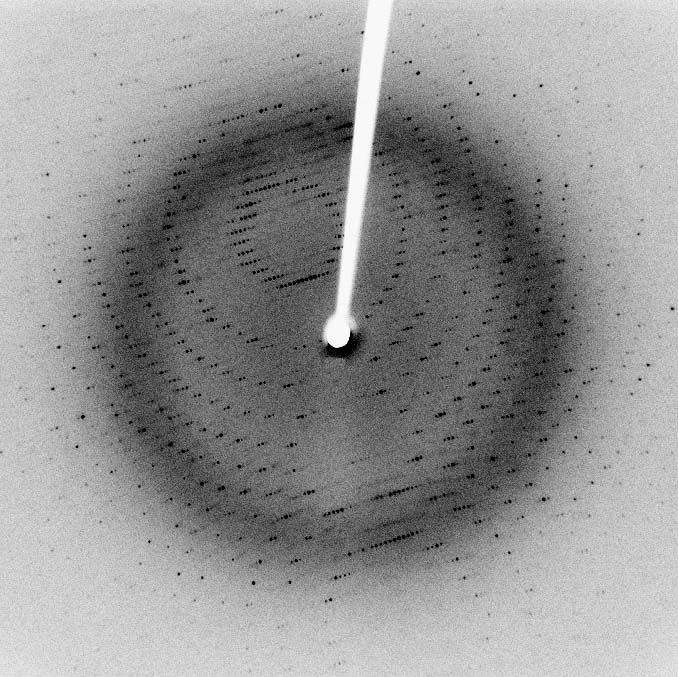
\includegraphics[width=0.3\textwidth]{figures/X-ray_diffraction_pattern_3clpro.jpg}
	\caption{\scriptsize Spettro di diffrazione da un cristallo di proteina.}
	\label{fig:diffrazione-proteina}
\end{figure}
Una volta ottenuta una misura del reticolo reciproco possiamo risalire al reticolo diretto faccendo il reciproco del reciproco.

\subsection{Teorema di Bloch}
\label{subsec:Teorema di Block}
Dalle definizioni date nei paragrafi precedenti possiamo scrivere le proprietà di periodicità del potenziale $U_c$ come:
\[
	U_c(\bs{r}+\bs{R}) = U_c(\bs{r})
.\]
Le autofunzioni di un potenziale periodico le possiamo trovare con il teorema di Bloch.
\begin{fact}[Teorema di Bloch]{def:Teorema di Bloch}
	Le autofunzioni di un potenziale periodico le possiamo identificare con il 
	prodotto di un'onda piana moltiplicata per una funzione periodica
	$u_{n\bs{k}}(\bs{r})$ avente lo stesso periodo del reticolo. 
	\[
		\psi_{n\bs{k}}(\bs{r}) = e^{i\bs{k}\cdot\bs{r}}u_{n\bs{k}}(\bs{r})
	.\] 
	Dove $\bs{k}$ è l'autovalore, diverso dal vettore $\bs{K}$ del reticolo reciproco.
\end{fact}
\subsubsection{Operatore di traslazione}
\label{subsubsec:Operatore di traslazione}

Un altro modo di esprimere il teorema è quello di dire che:
\[
	\psi_{n\bs{k}}(\bs{r}+\bs{R}) = e^{i\bs{k}\cdot\bs{R}} \psi_{n\bs{k}}(\bs{r})
.\] 
Dove ovviamente $\bs{R}$ è sempre un vettore del reticolo diretto. Da quest'ultima proprietà di traslazione se ne deduce che le autofunzioni del teorema di Bloch sono anche autostati delle traslazioni $T_{\bs{R}}$:
\[
	T_{\bs{R}}f(\bs{r}) = f(\bs{r}+\bs{R})
.\] 
Una regola di composizione per questo operatore è la seguente:
\[
	T_{\bs{R}}T_{\bs{R}'}=T_{\bs{R}+\bs{R}'}
.\] 
Tale operatore commuta con l'Hamiltoniana essendo questa periodica:
\[\begin{aligned}
	T_{\bs{R}}H\psi 
	=&
	H(\bs{r}+\bs{R})\psi(\bs{r}+\bs{R}) =\\
	=&
	H(\bs{r})\psi(\bs{r}+\bs{R})=\\
	=& HT_{\bs{R}}\psi(\bs{r})
.\end{aligned}\]
Inoltre gli operatori di traslazione commutano anche tra di loro:
\[
	T_{\bs{R}}T_{\bs{R}'}\psi(\bs{r}) 
	= T_{\bs{R}'}T_{\bs{R}}\psi(\bs{r}) 
	= \psi(\bs{r}+\bs{R}+\bs{R}')
.\] 
Quindi tutti gli autostati della Hamiltoniana li posso scrivere anche come autostati delle traslazioni. Il teorema di Bloch deriva proprio dall'aver scelto come autostati della Hamiltoniana quelli del'operatore di traslazione.\\
\subsubsection{Dimostrazione del teorema di Bloch}
\label{subsubsec:Dimostrazione del teorema di Bloch}
Prendiamo una $\psi$ che sia autostato delle traslazioni:
\[
	T_{\bs{R}}\psi  = c(\bs{R})\psi
.\] 
Applichiamo a questa un altro operatore di traslazione:
\[\begin{aligned}
	T_{\bs{R}'}T_{\bs{R}}\psi 
	=&
	c(\bs{R})T_{\bs{R}'}\psi  =\\
	=&
	c(\bs{R})c(\bs{R}')\psi
.\end{aligned}\]
Per le proprietà dell'operatore di traslazione si ha anche che:
\[
	T_{\bs{R}+\bs{R}'} = c(\bs{R}+\bs{R}')\psi
.\] 
Quindi abbiamo una condizione sugli autovalori delle traslazioni:
\[
	c(\bs{R}+\bs{R}') = c(\bs{R})c(\bs{R}')
.\] 
Per i vettori primari che generano il reticolo possiamo sempre scrivere gli autovalori di traslazione come \footnote{È una scrittura generale, possiamo scriverli in questo modo una volta normalizzati}:
\[
	c(\bs{a}_i) = e^{2\pi i x_i}
.\] 
Dove $x_i$ è in generale un numero complesso.\\
Preso un generico vettore del reticolo:
\[
	\bs{R}=n_1\bs{a}_1+n_2\bs{a}_2+n_3\bs{a}_3
.\] 
L'autovalore associato a questa traslazione sarà:
\[
	c(\bs{R})=e^{i\bs{k}\bs{R}}=c(\bs{a}_1)^{n_1}c(\bs{a_2})^{n_2}c(\bs{a}_3)^{n_3}
.\] 
Dove $\bs{k}$ è un vettore del tipo:
\[
	\bs{k}= x_1\bs{b}_1+x_2\bs{b}_2+x_3\bs{b}_3
.\] 
I $\bs{b}_i$ sono gli stessi del reticolo reciproco:
\[
	\bs{b}_i\bs{a}_j= 2\pi\delta_{ij}
.\] 
Gli autovalori del nostro operatore di traslazione gli possiamo quindi scrivere come:
\[
	T_{\bs{R}}\psi= c(\bs{R})\psi=e^{i\bs{k}\bs{R}}\psi(\bs{r}) \label{eq:quasi-bloch}
.\] 
Questa è la forma del teorema di Bloch, dobbiamo dimostrare che i $\bs{k}$ sono vettori reali, non vettori complessi generici. Per far questo dobbiamo introdurre delle condizioni al contorno sugli autostati: scegliamo le condizioni al contorno di Born Von Kauman.\\
\begin{defn}[Condizioni al contorno di Born Von Kauman]{def:Condizioni al contorno di Born Von Kauman}
	Condizioni periodiche sugli autostati:
	\[
	\psi(\bs{r}+N_i\bs{a}_i)=\psi(\bs{r})
	.\]
	Dove $N_i$ è il numero di celle nella direzione i-esima.
\end{defn}
Inserendo tale condizione al contorno nella \ref{eq:quasi-bloch} otteniamo che:
\[
	\psi_{n\bs{k}}(\bs{r}+N_i\bs{a}_i)
	= \underbrace{e^{iN_i\bs{k}\cdot\bs{a}_i}}_{=1 \text{ Per BVK}}
	\psi_{n\bs{k}}(\bs{r})
.\] 
Di conseguenza abbiamo che 
\[
	e^{iN_i\bs{k}\cdot\bs{a}_i}=1 
.\] 
Questo comporta che gli $x_i$ del vettore $\bs{k}$ sono vincolati ad essere numeri reali del tipo:
\[
	x_i = \frac{m_i}{N_i}
.\] 
Con $m_i$ interi. Possiamo anche riscrivere tale vettore $\bs{k}$ come:
\[
	\bs{k}=\sum_{i=1}^{3} \frac{m_i}{N_i}\bs{b}_i
.\] 
Ed il teorema di Bloch è così dimostrato.\\
Abbiamo inoltre il risultato che i vettori $\bs{k}$ gli possiamo descrivere all'interno dello spazio $\bs{K}$ del reticolo reciproco. Ad esempio considerando il caso di reticolo cubico si ha che, essendo $m_i$ interi e $N$ uguale per tutti i lati del reticolo diretto, dentro ad una cella unitaria del reticolo reciproco vi staranno $N$ vettori $\bs{k}$ per ognuna delle 3 direzioni. Tale situazione è rappresentata in Figura \ref{fig:vettori-k-nello-spazio-del-reticolo-reciproco-k} (o meglio, c'è un disperato tentativo di rappresentazione) partendo dal reticolo di Brilloiun.
\begin{figure}[ht]
    \centering
    \incfig{vettori-k-nello-spazio-del-reticolo-reciproco-k}
    \caption{Vettori k nello spazio del reticolo reciproco K}
    \label{fig:vettori-k-nello-spazio-del-reticolo-reciproco-k}
\end{figure}
In conclusione $\bs{k}$ è l'autovalore delle traslazioni e ci identifica gli autostati di Bloch nel potenziale periodico, da non confondere con i $\bs{K}$ che sono i vettori del reticolo reciproco.\\
Avendo scritto la funzione d'onda come
\[
	\psi(\bs{r})= e^{i\bs{k}\cdot\bs{r}}u(\bs{r}) \label{eq:onda-bloch}
.\] 
Si ha che un caso particolare di questo tipo di funzioni d'onda è l'onda piana:
\[
	\psi(\bs{r})=e^{i\bs{k}\cdot\bs{r}}
.\] 
Per questo caso, che è quello di particella libera, la periodicità della $u(\bs{r})$ è completa: per qualunque vettore $\bs{R}$ dello spazio "reale" abbiamo una $\psi$ periodica.\\
Questo ci fa capire che nel caso generale (quello con $u(\bs{r})$) ho una invarianza traslazionale (come nel caso di particelle libere) che è ridotta dalla presenza del solido che con il suo reticolo periodico influenza la funzione d'onda con il termine $u(\bs{r})$.\\
Siamo allora tentati di identificare il $\bs{k}$ che compare nella \ref{eq:onda-bloch} come il vettore d'onda dell'elettrone all'interno del solido \footnote{Non ci dobbiamo scordare che abbiamo trovato le autofunzioni dell'operatore di traslazione, sono le stesse della Hamiltoniana che descriveva il moto di un elettrone all'interno del solito!}.\\
Tuttavia non abbiamo più la completa invarianza traslazionale, quindi le funzioni d'onda di Bloch non sono autostati dell'impulso:
\[\begin{aligned}
	\bs{P} 
	&=
	\frac{\hbar \nabla}{i}\psi_{n\bs{k}}=\\
	=&
	\hbar \bs{k}\psi_{n\bs{k}}+
	\underbrace{e^{i\bs{k}\cdot\bs{r}}\nabla u_{n\bs{k}}(\bs{r})}_
	{\text{Pezzo di troppo}}
.\end{aligned}\]
In approssimazione semi-classica (scrivendo una equazione dinamica per l'elettrone) è possibile utilizzare $\hbar \bs{k}$ come se fosse ancora collegato con l'impulso dell'elettrone, ad esempio in risposta ad un campo elettrico esterno si può può trattare introducendo una accelerazione $\hbar \dot{\bs{k}}$. In questo modo si può ancora trattare questo come impulso, soltanto che quest'ultimo sarà definito a meno di un vettore $\bs{K}$ del reticolo reciproco\ldots\\
La conservazione dell'impulso a meno di un vettore del reticolo reciproco ha un significato interessante nella descrizione degli autostati per il nostro potenziale periodico:
\[
	\psi_{n\bs{k}}=e^{i\bs{k}\cdot\bs{r}}u_{n\bs{k}}(\bs{r})
.\] 
Possiamo chiederci se il modo di scrivere questo autostato sia unico, proviamo a fare il seguente cambio di variabile:
\[
	\bs{k}\to \bs{k}'+\bs{K} \label{eq:relazione-k}
.\] 
Questo equivale a supporre che il mio $\bs{k}$ sia fuori dalla cella unitaria (assumendo ovviamente che $\bs{k}'$ sia all'interno del reticolo reciproco invece). In questo modo l'autofunzione $\psi$ diventa:
\[
	\psi(\bs{r})= e^{i\bs{k}'\cdot\bs{r}}
	\underbrace{e^{i\bs{K}\cdot\bs{r}}u_{n\bs{k}}(\bs{r})}_
	{\substack{\text{Periodico con}\\ \text{la periodicità}\\ \text{del reticolo}}}
.\] 
Il secondo pezzo può essere infatti riscritto come:
\[
	e^{i\bs{K}\cdot\left( \bs{r}+\bs{R} \right) }u_{n\bs{k}}(\bs{r}+\bs{R}) =
	e^{i\bs{K}\cdot\bs{r}}\underbrace{e^{i\bs{K}\cdot\bs{R}}}_{=1}
	u_{n\bs{k}}(\bs{r})
.\] 
Inglobando la fase nella funzione periodica possiamo riscrivere:
\[
	\psi(\bs{r})= e^{i\bs{k}'\cdot\bs{r}}u_{n\bs{k}'}(\bs{r})
.\] 
Abbiamo allora una ridondanza nella individuazione del $\bs{k}$: la stessa $\psi$ può essere scritta come $\psi_{n\bs{k}}$ oppure come $\psi_{n\bs{k}'}$, ovvero con due onde piane diverse a moltiplicare la funzione periodica. \\
La cosa da ricordare è che questi vettori d'onda che sono la causa della ambiguita non sono scorrelati: sono legati per definizione da un $\bs{K}$ del reticolo reciproco come nella \ref{eq:relazione-k}.\\
Possiamo fare allora una cosa furba: possiamo descrivere tutti gli stati elettronici all'interno di una cella unitaria del reticolo reciproco, se sono fuori da tale cella basta traslare lo stato dentro a quest'ultima sfruttando l'ambiguita presente sui $\bs{k}$.\\
Tipicamente si descrivono gli autostati degli elettroni in un cristallo limitando i $\bs{k}$ delle autofunzioni di Bloch a stare dentro la prima zona di Brilloiun. I livelli energetici dipendono da $\bs{k}$, ad esempio nel caso di elettroni liberi si ha:
\[
	\mathcal{E}_{n\bs{k}}=
	\frac{\hbar^2\left|\bs{k}\right|^2}{2m}
.\] 
Plottando questi livelli ottengo delle curve come in Figura \ref{fig:livelli-energetici-di-una-particella-libera-in-un-potenziale-periodico}.
\begin{figure}[ht]
    \centering
    \incfig{livelli-energetici-di-una-particella-libera-in-un-potenziale-periodico}
    \caption{Livelli energetici di una particella libera in un potenziale periodico}
    \label{fig:livelli-energetici-di-una-particella-libera-in-un-potenziale-periodico}
\end{figure}
Questa è la struttura a bande del cristallo, il numero $n$ identifica la banda di energia a cui appartiene l'elettrone. \\
Dentro al cristallo non avremo il potenziale $U$ nullo, quindi non potremo considerare gli elettroni completamente liberi, questo modificherà la forma degli stati. In particolare vedremo che le degenerazioni (presenti ai bordi in Figura \ref{fig:livelli-energetici-di-una-particella-libera-in-un-potenziale-periodico}) verranno eliminate da questo potenziale cristallino.\\
Possiamo approfondire meglio il concetto di degenerazioni nella Figura \ref{fig:degenerazioni-nella-struttura-a-bande}.
\begin{figure}[H]
    \centering
    \incfig{degenerazioni-nella-struttura-a-bande}
    \caption{Degenerazioni nella struttura a bande}
    \label{fig:degenerazioni-nella-struttura-a-bande}
\end{figure}
\noindent
I due punti cerchiati sono i valori di $\bs{k}$ per cui si ha la degenerazione (nel caso in figura si mette in evidenza la prima degenerazione, salendo se ne incontrano altre).
